\pagestyle{fancy}
\section{Methodology}

\subsection{Research Design}
This project adopts a Design Science Research (DSR) approach because its primary goal is not only to study an existing phenomenon, but to create and evaluate an artifact that addresses an identified design problem. The problem established in the literature is that current generative interfaces often fall at one of two extremes: either assistance is constrained to static interface structures, or entire experiences are dynamically generated in ways that can undermine predictability and continuity. In response, this project proposes a conceptual framework for ephemeral, task-scoped generative UI components intended to augment existing applications without disrupting user workflow. The methodological contribution therefore lies in developing a framework that translates ideas from prior work on ephemerality, generative UI, and interaction support into a form that can guide design decisions in a broader productivity context.

Following this DSR logic, the study proceeds in three connected stages. First, a conceptual framework is synthesised from the literature in order to define the taxonomy, lifecycle, and design principles of ephemeral interface components. Second, that framework is instantiated in a website artifact that serves as a research instrument, allowing the proposed ideas to be embodied in a controlled interactive environment. Third, the artifact is evaluated through a comparative user study that contrasts an original interface with an ephemeral condition on a single, bounded task. This sequence ensures that the evaluation is not detached from theory: the framework informs the design of the artifact, and the artifact in turn provides the basis for assessing whether ephemeral augmentation can improve task performance and user experience without introducing excessive intrusiveness.

\subsection{Conceptual Framework}
This study develops a conceptual framework for ephemeral, task-scoped generative UI components to guide both artifact design and evaluation. In one sentence, the framework specifies \emph{which temporary support roles may appear}, \emph{how those supports are triggered and withdrawn}, and \emph{which constraints keep them useful without destabilising the host interface}. Positioning the framework here in the methodology is important because it defines the concepts that the artifact operationalises and the criteria against which the two interface conditions are later compared.

The first element is a taxonomy of component roles. Rather than classifying components by visual form, such as whether they appear as a panel, popover, or inline element, the taxonomy classifies them by the function they serve within the workflow. Three roles are distinguished. \emph{Interpretive support} helps users understand context, available options, outputs, or likely consequences before acting. \emph{Refinement support} helps users steer or configure an intended action before commitment, for example by comparing alternatives or adjusting parameters. \emph{Task-execution support} helps users complete a bounded subtask inside the surrounding application without replacing the broader workflow. Framing these roles as a taxonomy is methodologically useful because it makes explicit what kind of assistance is being introduced in each scenario and avoids treating ephemeral behaviour as a single undifferentiated interface style.

\begin{figure}[htbp]
    \centering
    \resizebox{0.95\textwidth}{!}{%
    \begin{tikzpicture}[
        font=\small,
        box/.style={
            draw,
            rounded corners,
            align=center,
            text width=0.22\textwidth,
            minimum height=2.2cm,
            inner sep=6pt
        },
        topbox/.style={
            draw,
            rounded corners,
            align=center,
            minimum width=0.42\textwidth,
            minimum height=1.2cm,
            inner sep=6pt
        }
    ]

    \node[topbox] (root) {Ephemeral, task-scoped\\generative support};

    \node[box, below left=1.8cm and 2.75cm of root] (interpretive) {\textbf{Interpretive support}\\Helps users understand\\context, outputs, or\\likely consequences};
    \node[box, below=1.8cm of root] (refinement) {\textbf{Refinement support}\\Helps users compare or\\adjust options before\\commitment};
    \node[box, below right=1.8cm and 2.75cm of root] (execution) {\textbf{Task-execution support}\\Helps users complete a\\bounded subtask within\\the existing workflow};

    \draw[-] (root.south west) -- (interpretive.north);
    \draw[-] (root.south) -- (refinement.north);
    \draw[-] (root.south east) -- (execution.north);

    \end{tikzpicture}
    }
    \caption{Taxonomy of ephemeral, task-scoped generative support roles.}
    \label{fig:taxonomy}
\end{figure}

The second element is a lifecycle describing how an ephemeral component enters and leaves use. Alternative stage patterns can be found in the literature, ranging from the minimal logic of temporary appearance and disappearance to more scaffolded models in which users configure support before committing to an outcome. For this study, the most appropriate synthesis is a four-stage lifecycle of \emph{trigger}, \emph{instantiation}, \emph{interaction}, and \emph{dismissal}. A component is triggered when a clear user goal or contextual need is detected that is not adequately supported by the persistent interface alone. That trigger may be explicit, such as a user request for help, or inferred from local behavioural and contextual signals, but only when the resulting support remains low-risk, relevant, and easy to dismiss. The component is then instantiated as a temporary interface element embedded within the existing application rather than replacing the surrounding interface. During interaction, users inspect, steer, or complete the immediate subtask while remaining oriented within the primary workflow. Finally, the component is dismissed once the task is completed, abandoned, or no longer contextually relevant. This lifecycle was selected because it retains the conceptual clarity of ephemerality while remaining concrete enough to implement as a state-based interaction model in the artifact.

\begin{figure}[htbp]
    \centering
    \resizebox{0.95\textwidth}{!}{%
    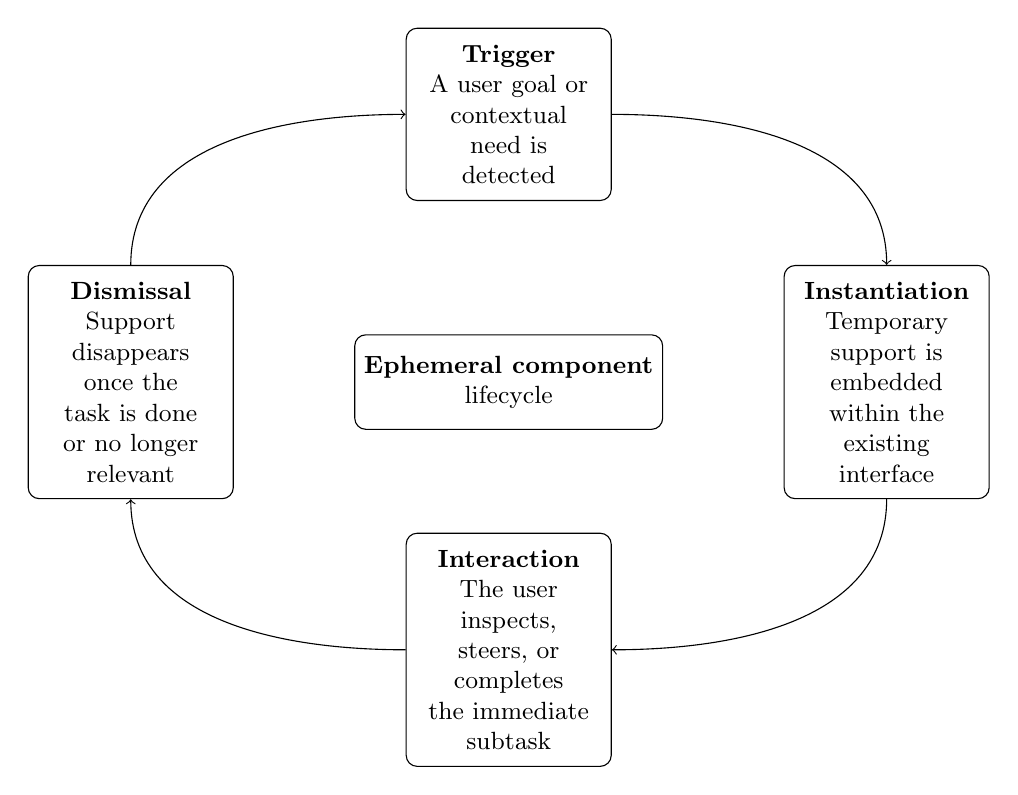
\begin{tikzpicture}[
        font=\small,
        stage/.style={
            draw,
            rounded corners,
            align=center,
            text width=0.18\textwidth,
            minimum height=2.0cm,
            inner sep=6pt
        }
    ]

    \node[draw, rounded corners, align=center, minimum width=3.4cm, minimum height=1.2cm] (core) at (0,0) {\textbf{Ephemeral component}\\lifecycle};

    \node[stage] (trigger) at (0,3.4) {\textbf{Trigger}\\A user goal or\\contextual need is\\detected};
    \node[stage] (instantiation) at (4.8,0) {\textbf{Instantiation}\\Temporary support is\\embedded within the\\existing interface};
    \node[stage] (interaction) at (0,-3.4) {\textbf{Interaction}\\The user inspects,\\steers, or completes\\the immediate subtask};
    \node[stage] (dismissal) at (-4.8,0) {\textbf{Dismissal}\\Support disappears\\once the task is done\\or no longer relevant};

    \draw[->] (trigger.east) to[out=0,in=90] (instantiation.north);
    \draw[->] (instantiation.south) to[out=-90,in=0] (interaction.east);
    \draw[->] (interaction.west) to[out=180,in=-90] (dismissal.south);
    \draw[->] (dismissal.north) to[out=90,in=180] (trigger.west);

    \end{tikzpicture}
    }
    \caption{Lifecycle of an ephemeral, task-scoped generative UI component: trigger, instantiation, interaction, and dismissal.}
    \label{fig:lifecycle}
\end{figure}

The third element is a set of design principles that constrain how ephemeral components should be introduced into an otherwise stable interface. Five principles guide the framework. \emph{Contextual relevance} means support should appear only when it serves a clear task-related purpose in the current situation. \emph{Bounded scope} means support should remain limited to the immediate subtask rather than taking over the larger workflow. \emph{Interface continuity} means the temporary component should preserve the surrounding page structure and the user's sense of place, rather than redirecting the interface toward an unrelated experience. \emph{User control} means users should be able to inspect, refine, confirm, or dismiss the support rather than being forced into a system decision. \emph{Graceful disappearance} means the component should recede cleanly once it is no longer needed. When support is inferred rather than explicitly invoked, these principles impose an additional safety constraint: inferred assistance may suggest or preload options, but it should not perform destructive or strongly consequential actions without explicit user confirmation. Together, these principles translate the theoretical idea of ephemerality into practical design criteria that can be applied consistently during artifact development and later assessed in the evaluation.

\subsection{Artifact Development}
The artifact developed in this project is a website used as a research instrument for evaluating the proposed framework in a controlled but realistic interaction setting. Rather than building a fully autonomous or fully generative application, the website is designed to preserve a recognisable baseline interface while allowing ephemeral, task-scoped components to be introduced at selected moments. This makes it possible to test whether the framework can augment an existing user experience without replacing the primary workflow altogether.

To operationalise the framework, the website will implement two interface conditions: an original condition representing the baseline experience and an ephemeral condition in which temporary, task-scoped components are introduced according to the taxonomy, lifecycle, and design principles defined above. The original condition will present the underlying tasks using a conventional persistent interface, whereas the ephemeral condition will surface temporary interface elements only when a user reaches a context in which additional guidance, refinement, or task support is needed. In this way, the comparison isolates the effect of ephemeral augmentation against the non-ephemeral alternative.

The website presents one scenario that represents a bounded productivity task within the application: a short presentation-refinement exercise foregrounding \emph{refinement support}. Participants receive a small slide deck and must improve its narrative order and clarify the problem slide before finalising it. The lifecycle of trigger, instantiation, interaction, and dismissal is implemented as the common interaction logic for both interface conditions. In the ephemeral condition, temporary support may propose grouping cues, comparisons, or lightweight controls that help the user adjust ordering and wording before commitment. Success is defined as producing a revised outline and problem statement that satisfy predefined task checks.

Although the ephemeral condition is allowed to be visually and structurally expressive, that expressiveness remains bounded by the framework. Temporary support may add task-relevant interface elements, annotate or highlight existing content, expose comparison views, or locally reconfigure a small region of the page. However, it does not replace the full application, arbitrarily reorganise the entire interface, or perform consequential actions without confirmation. In practice, the role category, lifecycle, task goals, and success criteria are fixed in advance, while local details such as wording, defaults, and the exact form of low-risk support may vary in response to immediate context. The ephemeral version is therefore not intended to be wholly different for every participant. Instead, it is constrained adaptation: users encounter the same scenario structures and the same framework rules, but the temporary support may be parameterised slightly differently within those limits. This preserves analytical robustness while still allowing the artifact to reflect the broader motivation of adaptive, goal-relevant ephemeral interfaces.

\subsection{Evaluation Design}

\subsubsection{Experimental Design}
The framework will be evaluated through a comparative within-subjects user study using the website artifact described above. Each participant will complete two trials in total: the same slide-refinement scenario once under the original baseline condition and once under the ephemeral condition, in an order randomised per participant. A within-subjects design is appropriate because it allows each participant to act as their own control, thereby reducing the influence of individual differences in digital literacy, task strategy, or prior familiarity with similar interfaces. Trial order will be randomised within the website so that participants encounter both conditions without a systematic sequence bias.

\subsubsection{Participants}
Participants will be recruited as regular users of web-based applications who can complete common digital tasks in a desktop browser environment. Recruitment will follow a convenience sampling approach appropriate to the scope of the capstone project. Inclusion criteria will focus on participants who are able to use standard web interfaces independently, while any exclusion criteria will be limited to factors that would prevent valid completion of the study tasks. The final sample size will depend on recruitment feasibility, but the study is designed to support repeated-measures comparisons between the two interface conditions.

\subsubsection{Materials and Procedure}
The primary study material is the experimental website, which implements both the original and ephemeral interface conditions. Participants will complete one bounded scenario twice: a presentation-style refinement task in which they adjust slide order and clarifying text. The task structure, goals, and success criteria remain constant for all users so that the study remains comparable across sessions. Within that shared structure, the ephemeral condition may vary in how temporary support is presented so that the assistance can respond to local context while remaining constrained by predefined design rules derived from the framework. In other words, the study does not test unlimited personalisation or unrestricted interface takeover. It tests bounded interface adaptation in which temporary support may add, highlight, compare, or locally rearrange elements while preserving interface continuity and user control.

The procedure will be fully website-based. After opening the study website, participants will read the study information, provide consent, and complete a short background questionnaire about their comfort with websites and familiarity with AI-assisted tools. The website will then present two task trials in a randomised order, representing the same scenario under the original baseline and ephemeral conditions. Before each trial, participants will receive a short task prompt that labels the interface version for fair debriefing. During each trial, the website will automatically log behavioural data. After each trial, participants will complete brief ratings on intrusiveness, perceived control, and helpfulness. After both trials are complete, participants will answer a final comparative questionnaire about overall preference between the two conditions, with an explicit reminder of which version corresponded to assistance for that participant. This fully instrumented procedure keeps the study structure consistent while allowing all behavioural and self-reported data to be collected in the same environment.

\subsubsection{Measures}
The evaluation combines behavioural and self-reported measures in order to capture both task performance and perceived experience. Behavioural measures are derived from interaction logs recorded by the website, while subjective measures are collected through short post-trial and post-study questionnaires. The core claim being tested is not simply that ephemeral interfaces are preferred, but that they can improve task support without introducing additional disruption. To assess that claim, the study will measure efficiency through task completion time, effectiveness through task completion rate, friction through interaction count, and user experience through ratings of intrusiveness, perceived control, helpfulness, and overall preference. In addition, ephemeral-only interaction logs will record whether temporary support was opened, used, refined, dismissed, or ignored, allowing the study to interpret how participants actually engaged with the generated assistance.

\begin{table}[htbp]
    \centering
    \caption{Dependent measures and collection methods.}
    \label{tab:measures}
    \begin{tabular}{@{}llll@{}}
        \toprule
        Measure & Type & Collection & Analysis \\
        \midrule
        Task completion rate & Binary & Event logging & Paired categorical comparison \\
        Task completion time & Continuous & Timestamps & Paired comparison \\
        Interaction count & Discrete & Event logging & Paired comparison \\
        Intrusiveness & Ordinal (1--7) & Post-trial Likert item & Paired comparison \\
        Perceived control & Ordinal (1--7) & Post-trial Likert item & Paired comparison \\
        Helpfulness & Ordinal (1--7) & Post-trial Likert item & Paired comparison \\
        Preference & Nominal & Final forced choice & Comparative choice analysis \\
        \bottomrule
    \end{tabular}
\end{table}

\subsubsection{Data Collection}
Data collection will combine instrumented event logging with questionnaire responses. For each trial, the website will record task start and end times, completion outcomes, interaction counts, and the active interface condition. In the ephemeral condition, additional logs will capture component trigger events, support openings, dismissals, confirmations, and refinement actions. Post-trial survey items will capture perceived intrusiveness, perceived control, and helpfulness, while the final questionnaire will capture overall preference between conditions. To link behavioural and survey data, each session will be associated with a participant identifier that is stored consistently across the website logs and questionnaire responses.

\subsubsection{Analysis Plan}
The primary analysis will compare the original and ephemeral conditions on each dependent measure using repeated-measures statistical tests appropriate to the data type and distribution. Task completion rate will be analysed as a paired categorical outcome, while time, interaction count, and subjective ratings will be analysed using paired comparisons, with non-parametric alternatives considered if distributional assumptions are not met. Preference will be analysed as a comparative choice measure. Ephemeral-only interaction logs will be analysed descriptively to show whether support was typically accepted, refined, or dismissed, which helps interpret whether a null or positive effect reflects the quality of the support itself or low uptake. The analysis will therefore focus on whether the ephemeral condition yields improvements in efficiency, effectiveness, or perceived helpfulness without increasing intrusiveness or reducing perceived control. Because the ephemeral experience may vary within bounded framework rules, the analysis treats that variation as part of the intended adaptive behaviour of the artifact rather than as an uncontrolled change to the task itself.